\chapter{Analiza wyników}
Program był tworzony, testowany oraz wykonywany na komputerze posiadającym 4 rdzeniowy procesor Intel Core i7-6700HQ oraz pamięć 8 GB (SO-DIMM DDR4, 2133MHz).

\section{Wygenerowane wykresy}
\label{wynik:wykres}
W celu analizy otrzymanych danych, program został uruchomiony pewną ilość razy, za każdym razem z innymi danymi wejściowymi. Otrzymane wykresy przedstawiają zmianę ilości elektronów znajdujących się w pułapkach w czasie trwania symulacji.

\begin{figure}[H]
\centering

\includegraphics[width=17cm, height = 10cm]{q}
\caption{Ilość elektronów: $20^{4}$, ilość dziur elektronowych: $30^{4}$, zakres w którym losowane są położenia cząstek: [-1000,1000], symulowany czas: 1000 dni. Czas wykonywania symulacji: DO DODANIA JESLI SIE WYGENERUJE, JAK NIE DAC MNIEJSZE}
\end{figure}

\begin{figure}[H]
\centering
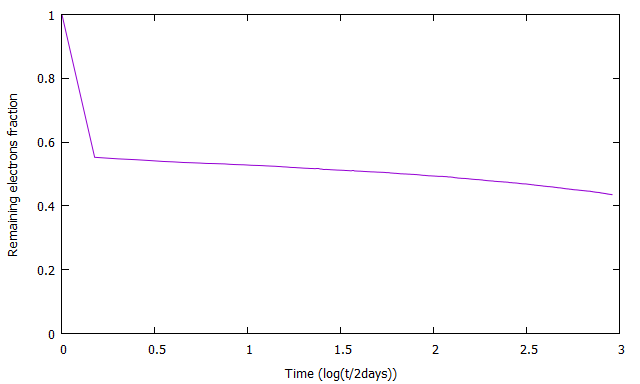
\includegraphics[width=17cm, height = 10cm]{wykres2}
\caption{Ilość elektronów: $10^{4}$, ilość dziur elektronowych: $10^{4}$, zakres w którym losowane są położenia cząstek: [-900,900], symulowany czas: 5 lat. Czas wykonywania symulacji: 13h}
\end{figure}
 
\begin{figure}[H]
\centering
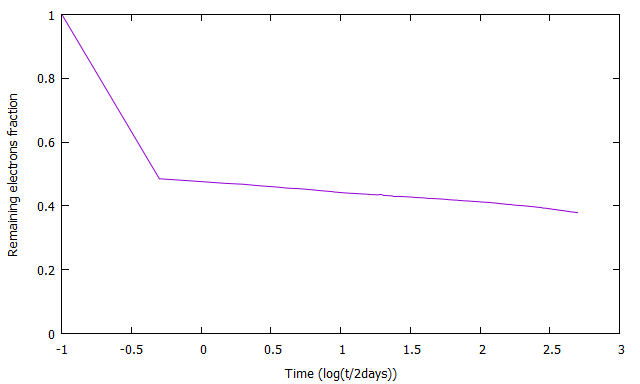
\includegraphics[width=17cm, height = 10cm]{wykres1}
\label{rys:1}
\caption{Ilość elektronów: $10^{4}$, ilość dziur elektronowych: $10^{4}$, zakres w którym losowane są położenia cząstek: [-800,800], symulowany czas: 1000 dni. Czas wykonywania symulacji: 3h}
\end{figure}

\begin{figure}[H]
\centering
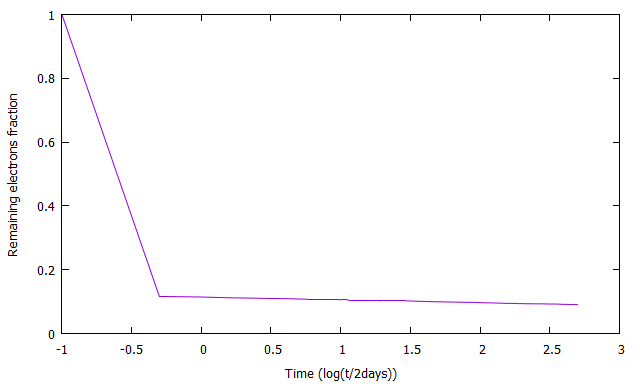
\includegraphics[width=17cm, height = 10cm]{wykres2_2}
\label{rys:2}
\caption{Ilość elektronów: $10^{4}$, ilość dziur elektronowych: $10^{4}$, zakres w którym losowane są położenia cząstek: [-400,400], symulowany czas: 1000 dni. Czas wykonywania symulacji: 5min}
\end{figure}




\begin{figure}[H]
\centering
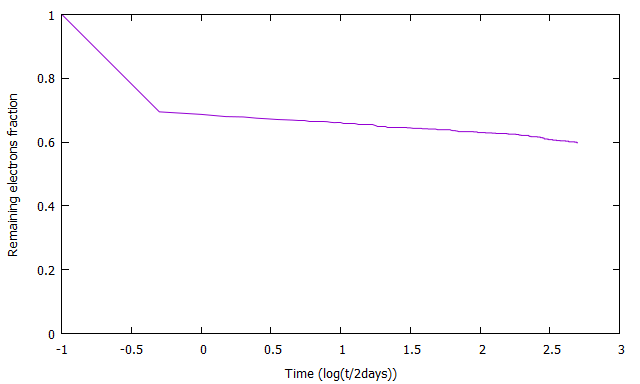
\includegraphics[width=17cm, height = 10cm]{wykres3}
\caption{Ilość elektronów: $10^{3}$, ilość dziur elektronowych: $10^{3}$, zakres w którym losowane są położenia cząstek: [-500,500], symulowany czas: 1000 dni. Czas wykonywania symulacji: 4min}
\end{figure}




\section{Analiza wykresów}
Analizując otrzymane wykresy można zauważyć znaczny spadek ilości elektronów w pułapkach na samym początku wykonywania programu. Jest to spowodowane faktem, że wszystkie współrzędne cząstek są losowane z podanego zakresu. Oznacza to, że na początku symulacji wiele pułapek elektronowych zawierających elektrony znajduje się bardzo blisko centrów rekombinacji. Powołując się na równania \ref{eq:1} oraz \ref{eq:2} obserwujemy, że odległość między pułapką a centrum rekombinacji znacząco wpływa na prawdopodobieństwo zajścia efektu tunelowego, co skutkuje zaobserwowanym początkowym spadkiem ilości wzbudzonych elektronów. Po wystąpieniu znaczącego spadku można zaobserwować, że ilość elektronów znajdujących się w pułapkach zaczyna maleć z dużo mniejszą częstotliwością. Wykres zaczyna wtedy przypominać funkcję liniową. Obrazuje to fakt występowania atermicznego zaniku luminescencyjnego, który zachodzi samoistnie dzięki zjawisku tunelowania, bez dostarczania dodatkowej energii. 

Ważnym parametrem symulacji jest zakres z którego losowane są wartości położenia dla cząstek. Porównując ze sobą wykresy \hyperref[rys:1]{rys.4.3} oraz \hyperref[rys:2]{rys. 4.4} gdzie ilość elektronów oraz symulowany czas są takie same, a zakres wartości położeń cząstki znacząco się różni, zaobserwowano, że im większa gęstość ładunków tym efekt tunelowania zachodzi szybciej, co jest zgodne z przewidywaniami wynikającymi ze wzoru \ref{eq:2}. Dzięki temu czas wykonania programu widocznie się zmniejszył z 3h do ok. 5min. 
